
\begin{frame}{‌مرتب‌سازی ادغامی}
\begin{itemize}\itemr
\item[-]
الگوریتم مرتب‌سازی ادغامی
\fn{1}{merge sort}
در دستهٔ الگوریتم‌های تقسیم و حل قرار می‌گیرد. با شروع از آرایهٔ
\code{A[1:n]}
، در هر مرحله یکی از زیر آرایه‌های
\code{A[p:r]}
مرتب می‌شود و سپس این زیر آرایه‌ها با یکدیگر ادغام می‌شوند تا آرایهٔ اصلی مرتب شود. برای هر یک از زیر آرایه‌ها، الگوریتم مرتب‌سازی ادغامی فراخوانی می‌شود و به همین نحو، آن زیر آرایه‌ها تقسیم شده و به روش بازگشتی مرتب می‌شوند.
\end{itemize}
\end{frame}


\begin{frame}{‌مرتب‌سازی ادغامی}
\begin{itemize}\itemr
\item[-]
مراحل انجام مرتب‌سازی ادغامی به صورت زیر است :
\item[۱.]
تقسیم : آرایهٔ
\code{A[p:r]}
به دو زیرآرایهٔ مساوی تقسیم می‌شود. اگر 
\code{q} 
وسط 
\code{p}
 و 
\code{r}
  باشد، آنگاه دو آرایهٔ به دست آمده عبارتند از
\code{A[p:q]}
و
\code{A[q+1:r]}
. در مرحلهٔ اول 
\code{p}
 برابر با 
\code{1}
  و 
\code{r}
   برابر است با 
\code{n} .
\item[۲.]
حل : الگوریتم به صورت بازگشتی برای دو زیر آرایهٔ
\code{A[p:q]}
و
\code{A[q+1:r]}
فراخوانی می‌شود.
\item[۳.]
ترکیب : با ادغام دو آرایهٔ
\code{A[p:q]}
و
\code{A[q+1:r]}
که هر دو مرتب شده هستند، آرایهٔ مرتب شدهٔ
\code{A[p:r]}
به دست می‌آید.
\end{itemize}
\end{frame}


\begin{frame}{‌مرتب‌سازی ادغامی}
\begin{itemize}\itemr
\item[-]
این الگوریتم به طور بازگشتی فراخوانی می‌شود تا به حالت پایه برسیم.
در حالت پایه، آرایهٔ به دست آمده شامل تنها یک عنصر است که در این حالت آرایه نیاز به مرتب‌سازی ندارد. در واقع هنگامی به حالت پایه می‌رسیم که 
\code{p}
 برابر با 
\code{r}
  باشد.
\item[-]
در مرحلهٔ ادغام، با فرض اینکه دو آرایهٔ به دست آمده مرتب شده هستند، دو آرایه باید به نحوی با یکدیگر ترکیب شوند که آرایهٔ به دست آمده مرتب شده باشد.
\end{itemize}
\end{frame}


\begin{frame}{‌مرتب‌سازی ادغامی}
\begin{itemize}\itemr
\item[-]
الگوریتم مرتب‌سازی ادغامی به صورت زیر است.
\begin{algorithm}[H]\alglr
  \caption{Merge Sort} 
  \begin{algorithmic}[1]
    \Func{Merge-Sort}{A, p, r}
    \If{p >= r}	\LeftComment{zero or one element?}
    	\State \Return
    \EndIf    
    \State q = $\lfloor$ (p+r)/2 $\rfloor$	\LeftComment{ midpoint of A[p:r]}
    \State Merge-Sort (A, p, q)	\LeftComment{ recursively sort A[p:q]}
    \State Merge-Sort (A, q+1, r)	\LeftComment{ recursively sort A[q+1:r]}
    \State Merge (A, p, q, r) \LeftComment{Merge A[p:q] and A[q+1:r] into A[p:r].}
  \end{algorithmic}
  \label{alg:merge-sort}
\end{algorithm}
\end{itemize}
\end{frame}

\begin{frame}{‌مرتب‌سازی ادغامی}
\begin{itemize}\itemr
\item[-]
برای ادغام دو زیرآرایه از الگوریتم زیر استفاده می‌کنیم.
\begin{algorithm}[H]\alglr
  \caption{Merge Sort} 
  \begin{algorithmic}[1]
    \Func{Merge}{A, p, q, r}
    \State nl = q - p + 1 \LeftComment{ length of A[p:q]}
    \State nr = r - q \LeftComment{ length of A[q+1 : r]}
    \State let L[ 0 : nl - 1 ] and R[ 0 : nr - 1 ] be new arrays
    \For{i = 0 \To nl - 1} \LeftComment{ copy A[p:q] into L[0:nl - 1]}
      \State L[i] = A[p+i]
    \EndFor
    \For{j = 0 to nr - 1} \LeftComment{copy A[q+1:r] into L[0:nr - 1]} 
      \State R[j] = A[q + j + 1]
     \EndFor
  \end{algorithmic}
  \label{alg:merge}
\end{algorithm}
\end{itemize}
\end{frame}


\begin{frame}{‌مرتب‌سازی ادغامی}
\begin{itemize}\itemr
\item[-]
\begin{algorithm}[H]\alglr
  \caption{Merge Sort} 
  \begin{algorithmic}[1]
  \setcounter{ALG@line}{7}
    \Func{Merge}{A, p, q, r}
      \State i = 0 \LeftComment{ i indexes the smallest remaining element in L}
      \State j = 0 \LeftComment{j indexes the smallest remaining element in R}
      \State k = p \LeftComment{ k indexes the location in A to fill}
    \newline\LeftComment{ As long as each of the arrays L and R contains un unmerged element, copy the smallest unmerged element back into A[p : r].}                              
    \While{ i < nl \Aand j < nr}
          \If {L[i] <= R[j]}
              \State A[k] = L[i]
              \State i = i + 1
          \Else 
              \State A[k] = R[j]
              \State j = j + 1
           \EndIf
          \State k = k + 1
      \EndWhile
  \end{algorithmic}
  \label{alg:merge}
\end{algorithm}
\end{itemize}
\end{frame}



\begin{frame}{‌مرتب‌سازی ادغامی}
\begin{itemize}\itemr
\item[-]
\begin{algorithm}[H]\alglr
  \caption{Merge Sort} 
  \begin{algorithmic}[1]
    \setcounter{ALG@line}{18}
    \Func{Merge}{A, p, q, r}
    \newline\LeftComment{ Having gone through one of L and R entirely, copy the  remainder of the other to the end of A[p:r]}                                    
    \While{i < nl}
             \State A[k] = L[i]
             \State i = i + 1
             \State k = k + 1
     \EndWhile      
    \While{ j < nr}
            \State A[k] = R[j]
            \State j = j + 1
            \State k = k + 1 
      \EndWhile                                             
  \end{algorithmic}
  \label{alg:merge}
\end{algorithm}
\end{itemize}
\end{frame}


\begin{frame}{‌مرتب‌سازی ادغامی}
\begin{itemize}\itemr
\item[-]
یک مثال از ادغام دو زیر آرایه در شکل زیر نشان داده شده‌است.
\begin{figure}
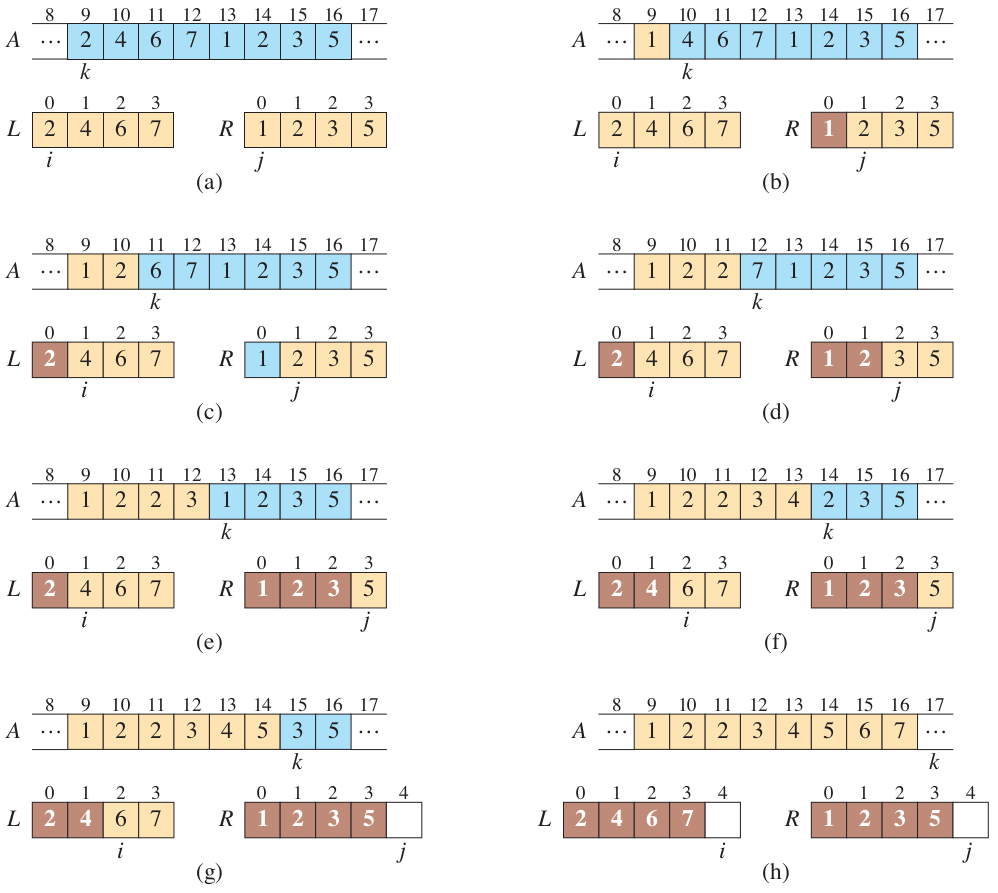
\includegraphics[width=0.5\textwidth]{figs/chap03/merge-example}
\end{figure}
\end{itemize}
\end{frame}


\begin{frame}{‌مرتب‌سازی ادغامی}
\begin{itemize}\itemr
\item[-]
در حلقهٔ تکرار الگوریتم ادغام، در هر تکرار یکی از عناصر در آرایهٔ A کپی می‌شوند و در کل تا پایان الگوریتم n عنصر در آرایه کپی می‌شوند، پس زمان اجرای این الگوریتم
\ath{n}
است.
\end{itemize}
\end{frame}


\begin{frame}{‌مرتب‌سازی ادغامی}
\begin{itemize}\itemr
\item[-]
یک مثال مرتب‌سازی ادغامی در شکل زیر نشان داده شده‌است.
\begin{figure}
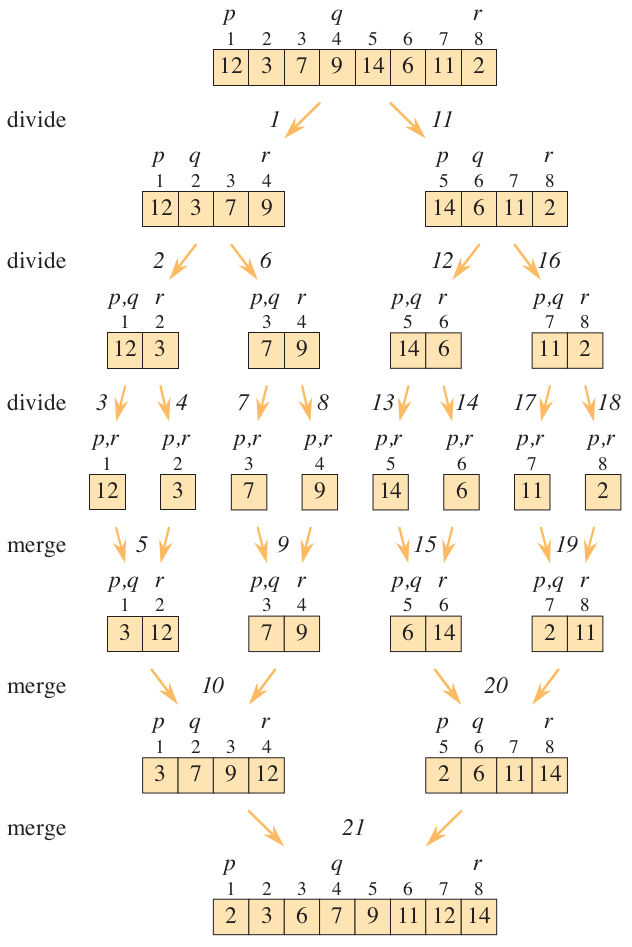
\includegraphics[width=0.3\textwidth]{figs/chap03/merge-sort-example}
\end{figure}
\end{itemize}
\end{frame}


\begin{frame}{‌مرتب‌سازی ادغامی}
\begin{itemize}\itemr
\item[-]
وقتی یک مسئله به صورت بازگشتی طراحی می‌شود، زمان اجرای آن را نیز معمولا با استفاده از معادلات بازگشتی
\fn{1}{recurrence equation}
به دست می‌آوریم.
در این معادلات بازگشتی، زمان اجرای یک الگوریتم با ورودی اندازهٔ n توسط زمان اجرای همان الگوریتم با ورودی‌هایی از اندازه‌های کوچک‌تر به دست می‌آید. روش‌های متعددی برای حل مسائل بازگشتی وجود دارند که می‌توان از آنها استفاده کرد.
\end{itemize}
\end{frame}


\begin{frame}{‌مرتب‌سازی ادغامی}
\begin{itemize}\itemr
\item[-]
به طور کلی اگر فرض کنیم زمان اجرای یک الگوریتم برای ورودی با اندازهٔ n برابر با
\m{T(n)}
باشد و توسط روش تقسیم و حل مسئلهٔ مورد نظر به
\m{a}
زیر مسئله تقسیم شود که اندازه ورودی هر کدام
\m{n/b}
باشد، آنگاه به زمان
\m{aT(n/b)}
برای حل مسئله نیاز داریم.
\item[-]
همچنین اگر به زمان 
\m{D(n)}
 برای تقسیم مسئله به زیر مسئله‌ها و به زمان
\m{C(n)} 
 برای ادغام زیر مسئله‌ها نیاز داشته باشیم، آنگاه این زمان‌ها به زمان مورد نیاز برای حل مسئله افزوده می‌شوند.
\end{itemize}
\end{frame}


\begin{frame}{‌مرتب‌سازی ادغامی}
\begin{itemize}\itemr
\item[-]
فرض کنید در حالت پایه، یعنی وقتی اندازهٔ ورودی از یک مقدار معین کوچکتر است، اجرای برنامه در زمان ثابت انجام شود، یعنی زمان اجرای برنامه در حالت پایه به اندازهٔ ورودی n بستگی نداشته باشد.
\item[-]
در حالت کلی زمان اجرای یک الگوریتم تقسیم و حل را می‌توانیم با استفاده از رابطهٔ بازگشتی زیر بنویسیم.
\begin{align*}
\m{T(n)} = \left\{\begin{array}{lr}
          \m{\Theta (1)}& \m{n < n_0}~\text{اگر}\\
          \m{D(n) + aT(n/b) + C(n)}&\text{در باقی حالات}
\end{array}\right.
\end{align*}
\end{itemize}
\end{frame}


\begin{frame}{‌مرتب‌سازی ادغامی}
\begin{itemize}\itemr
\item[-]
حال زمان اجرای الگوریتم مرتب‌سازی ادغامی را در بدترین حالت به ازای یک آرایهٔ با طول n تحلیل می‌کنیم.\\
۱. تقسیم : تقسیم کردن آرایه به دو قسمت در زمان ثابت انجام می‌شود، بنابراین داریم
\m{D(n) = \ath{1}} .\\
۲. حل : در مرحلهٔ حل از دو آرایه با اندازه
\m{n/2}
به صورت بازگشتی استفاده می‌کنیم بنابراین زمان مورد نیاز در این مرحله برابر است با
\m{2T(n/2)}
. توجه کنید که ممکن است آرایه بر دو بخش پذیر نباشد، اما معمولاً در تحلیل الگوریتم از توابع کف و سقف صرف نظر می‌کنیم، چرا که تأثیری در تحلیل الگوریتم نمی‌گذارند.\\
۳. ترکیب : در این مرحله برای ادغام دو آرایه، جهت تولید یک آرایه با طول n به زمان
\ath{n}
نیاز داریم، بنابراین داریم
\m{C(n) = \ath{n}} .
\end{itemize}
\end{frame}


\begin{frame}{‌مرتب‌سازی ادغامی}
\begin{itemize}\itemr
\item[-]
بنابراین در مجموع زمان اجرای الگوریتم مرتب‌سازی ادغامی به صورت زیر است :
\begin{center}
\m{T(n) = 2T(n/2) + \ath{n}}
\end{center}
\item[-]
با حل این معادله بازگشتی می‌توان به دست آورد
\m{T(n) = \ath{n \lg n}}
، بنابراین زمان مورد نیاز برای اجرای الگوریتم مرتب‌سازی ادغامی از مرتب‌سازی درجی بهتر است.
\end{itemize}
\end{frame}


\begin{frame}{‌مرتب‌سازی ادغامی}
\begin{itemize}\itemr
\item[-]
حال برای اینکه بدون حل معادله بازگشتی، زمان اجرای به دست آمده را درک کنیم، می‌توانیم الگوریتم را به صورت زیر تحلیل کنیم.
\item[-]
برای سادگی فرض می‌کنیم طول آرایهٔ ورودی برابر با n بوده و n توانی از ۲ است. با این ساده‌سازی همیشه با تقسیم n بر ۲ یک عدد صحیح به دست می‌آید.
\item[-]
زمان اجرای الگوریتم را به صورت زیر می‌نویسیم.
\begin{align*}
\m{T(n) =} \left\{\begin{array}{lr}
          \m{c_1} & \m{n = 1}~\text{اگر}\\
          \m{2T(n/2) + c_2n} & \m{n > 1}~ \text{اگر}\\
\end{array}\right.
\end{align*}
\item[-]
در اینجا
\m{c_1}
زمان اجرای الگوریتم است هنگامی که طول ورودی ۱ باشد و
\m{c_2}
مضرب ثابتی است که برای تقسیم و ادغام آرایه با طول n نیاز داریم.
\end{itemize}
\end{frame}


\begin{frame}{‌مرتب‌سازی ادغامی}
\begin{itemize}\itemr
\item[-]
شکل‌های زیر تقسیم این مسئله را به زیر مسئله‌ها و تحلیل زمان زیر مسئله‌ها را نشان می‌دهد.
\LR{
\begin{figure}
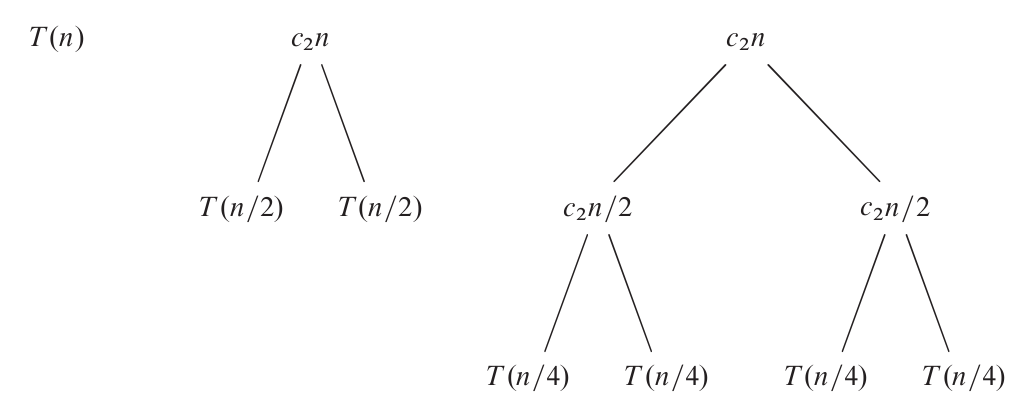
\includegraphics[width=0.5\textwidth]{figs/chap03/merge-sort-analysis1}
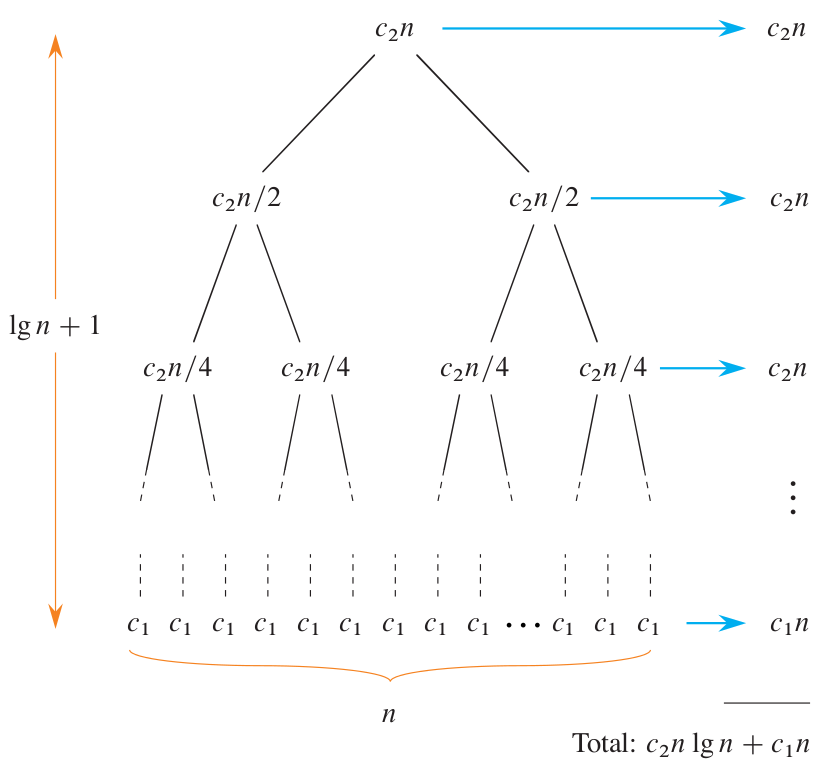
\includegraphics[width=0.4\textwidth]{figs/chap03/merge-sort-analysis2}
\end{figure}
}
\end{itemize}
\end{frame}


\begin{frame}{‌مرتب‌سازی ادغامی}
\begin{itemize}\itemr
\item[-]
مقدار
\m{c_2n}
در ریشهٔ این درخت در واقع زمان مورد نیاز برای تقسیم و ادغام را نشان می‌دهد، هنگامی که اندازهٔ مسئله برابر است با n . دو زیر درخت در سطح ۱ این درخت زمان‌های مورد نیاز را وقتی اندازهٔ ورودی
\m{n/2}
است نشان می‌دهند. هزینه مورد نیاز برای تقسیم و ادغام هر‌کدام از این زیر درخت‌ها برابر است با
\m{c_2n/2}
و مجموعه این هزینه‌ها برای دو زیر درخت برابر است با
\m{c_2n}.
\item[-]
چنانچه این محاسبات را ادامه دهیم، به این نتیجه می‌رسیم که هزینه تقسیم و ادغام برای هر یک از سطوح درخت برابر است با
\m{c_2n}.
\end{itemize}
\end{frame}


\begin{frame}{‌مرتب‌سازی ادغامی}
\begin{itemize}\itemr
\item[-]
سطح آخر، یعنی سطحی که برگ‌های درخت در آن قرار دارد، حالت پایه را نشان می‌دهد که در این حالت زمان اجرای هر یک از زیر آرایه‌ها برابر است با
\m{c_1}
و چون تعداد n زیر آرایه با طول ۱ داریم، زمان اجرا برای کل زیر آرایه‌ها برابر است با
\m{c_1 n}.
\item[-]
از آنجایی که این درخت در هر مرحله به دو بخش تقسیم می‌شود، تعداد سطوح درخت برابر است با
\m{\lg n + 1}.
\item[-]
بنابراین زمان کل اجرای الگوریتم برابر است با
\m{c_2n \lg n+ c_1n} .
\item[-]
می‌توانیم با استفاده از تحلیل مجانبی بنویسیم
\m{T(n) = \ath{n \lg n}}.
\end{itemize}
\end{frame}
